\documentclass{tfgitic}[2023/06/30]
% per a fórmules químiques
\usepackage[version=4]{mhchem}
% Per dibuixar gràfics: base general i gràfics senzills
\usepackage{tikz}
\usetikzlibrary{arrows, positioning, automata}
\tikzset{initial text=Inici, every state/.style={thick, fill=gray!10}}
% Per dibuixar gràfics: circuits electrònics
\usepackage[europeanresistors,americaninductors]{circuitikz}
% Per dibuixar gràfics: diagrames diversos
\usepackage{pgfplots}
% Per escriure algoritmes
\usepackage[plain,figure]{algorithm2e}
% Per a usar taules elàstiques
\usepackage{tabularx}

% Indica quines bd bibliografiques usarem
\addbibresource{tfg.bib}

% Marges en els algoritmes
\setlength{\algomargin}{4em}

% Versió de pgfplots a usar
\pgfplotsset{compat=newest}

\definecolor{tufte1}{rgb}{0.7,0.7,0.55}
\definecolor{yellowmarker}{HTML}{DEF440}

\pgfplotsset{
	tufte bar/.style={
		ybar,
		axis line style={draw opacity=0},
		xtick=\empty,
		ymin=0,
		bar width=3mm,
		x=2*\pgfkeysvalueof{/pgf/bar width},
		ymajorgrids,
		grid style=white,
		axis on top,
		major tick length=0pt,
		cycle list={
			fill=tufte1, draw=none\\
		},
		enlarge x limits={
			abs=0.5*\pgfkeysvalueof{/pgf/bar width}
		},
		axis x line*=bottom,
		x axis line style={
			draw opacity=1,
			tufte1,
			thick
		},
		yticklabel=\pgfmathprintnumber{\tick}\,\%
	}
}

\title{OsPlot: Com implementar osci\lgem oscopis amb un microcontrolador i Linux}

\subtitle{Una guia pràctica per a la creació d'un osci\lgem oscopi digital amb plataformes obertes}

\author{Joan Vilardaga Castro}

\advisor{Francisco Del Aguila López}

\dedication{Dedicació}

\begin{acknowledgments}
Tot el meu agraïment.
\end{acknowledgments}

\begin{resum}
En aquest document es descriu una guia que permeti a qualsevol persona
transformar un microcontrolador i un ordinador en un osci\lgem oscopi
funcional. Mitjançant l'ús de plataformes obertes com Linux, Arduino i
GNUPlot, aquesta investigació intenta oferir una solució de baix cost
i accessible per a gent interessada en l'anàlisi de senyals.
\end{resum}

\begin{abstract}
This document describes a guide that enables anyone to transform a
microcontroller and a computer into a functional oscilloscope By using
open platforms such as Linux, Arduino and GNUPlot, this research aims
to provide a low-cost and accessible solution for people interested in
signal analysis.
\end{abstract}

\begin{document}

\part{Memòria}

\chapter{Introducció}
\label{cap:intro}

\section{Origen del treball: Osci\lgem oscopi amb GNUPlot}
\label{sec:origen}

GNUPlot \cite{gnuplot} és un programa de traçat de gràfics en 2D i 3D
que permet visualitzar i analitzar diferents conjunts de dades. Tot i
que GNUPlot és una eina per fer gràfics estàtics, es pot combinar amb
altres programes o ``scripts'' per aconseguir la funcionalitat de
traçat en temps real.

És precisament aquest descobriment el que obre la porta a la
possibilitat de fer un osci\lgem oscopi amb GNUPlot com a plataforma
principal. Així, aquesta investigació s'enfoca a preparar una guia que
permeti crear un osci\lgem oscopi digital mitjançant GNUPlot.

\section{Objectius}
\label{sec:objectius}

\begin{enumerate}
	\item Evaluar la capacitat de GNUPlot per visualtizar dades en
          temps real.
	\item Desenvolupar OsPlot, una arquitectura genèrica per
          transformar un microcontrolador i un ordinador en un
          osci\lgem oscopi.
      \item Estendre l'arquitectura amb alternatives a GNUPlot.
	\item Implementar programes de referència que explotin les
          diferents possibilitats de l'arquitectura.
\end{enumerate}

\section{Com funciona un osci\lgem oscopi}
\label{sec:com-funciona-oscil·loscopi}

Un osci\lgem oscopi \cite{viqui-oscil·loscopi} és un instrument de
mesura que s'utilitza per visualitzar i analitzar senyals elèctrics
variables en el temps. Com amb moltes altres coses, els osci\lgem
oscopis són instruments que han evolucionat amb la digitalització,
creant una nova generació d'osci\lgem oscopis més precisos i que poden
fer operacions molt més complexes com mitges, pic a pic o
transformades ràpides de Fourier.

\subsection{Funcionament bàsic}
\label{subsec:funcionament-bàsic}

Els osci\lgem oscopis digitals es basen en l'ús d'un ADC (convertidor
analògic-digital), un sistema que converteix senyals analògics en
senyals digitals, les quals es processen per generar una representació
gràfica en temps real a la pantalla. L'eix horitzontal indica el
temps, i l'eix vertical indica generalment voltatge (tot i que es
poden mesurar altres magnituds com el corrent).

Tots els osci\lgem oscopis incorporen un subsistema de ``trigger''
\cite{funcionament-trigger} que té com a funció establir un punt de
referència i sincronitzar la captura de les dades. Aquest subsistema
és essencial per garantir una visualització estable i repetible. Sense
el ``trigger'', el senyal a visualitzar es desplaçaria constantment a
través de l'eix horitzontal, fent impossible la seva observació.

\subsection{Conceptes importants de senyals digitals}
\label{subsec:conceptes-pds}

Com que el treball se centra en osci\lgem oscopis digitals, és
necessari conèixer alguns dels conceptes claus del processament
digital del senyal \cite{llibre-pds}:

\begin{itemize}
	\item Senyal analògic (o continu): Tipus de senyal format per
          variables contínues. Encara que aquests valors estiguin
          confinats en un rang màxim i mínim, poden tenir una precisió
          infinita, no hi ha espais buits.
	\item Senyal digital (o discret): Seqüència de valors discrets
          separats en el temps. A diferència dels analògics, els
          senyals discrets tenen espais buits.
	\item Quantització: És el procés d'aproximar un valor continu
          al valor discret més proper. Sigui aproximació o truncament,
          sol introduir error de mesura, ja que un valor discret no
          pot representar els infinits decimals d'un valor continu.
	\item Resolució: És la diferència entre dos valors d'un rang
          discret. Determina el màxim error de discretització i el
          nombre de bits d'una mostra.
	\item Mostreig: Procés que transforma un senyal analògic en un
          senyal discret mitjançant l'ús repetit de la quantització.
          Cada valor quantitzat és una mostra del senyal analògic.
	\item Freqüència de mostreig: El nombre de mostres que captura
          un ADC cada segon. La màxima freqüència que podrà captar
          l'osci\lgem oscopi serà com a màxim la meitat de la
          freqüència de mostreig (criteri de Nyquist).
\end{itemize}

\chapter{OsPlot}

En aquest capítol primer s'explorarà la manera de convertir GNUPlot en
una eina per visualitzar dades en temps real. Seguidament, s'intentarà
dissenyar l'arquitectura més simple d'OsPlot, on una Arduino envia pel
port sèrie mostres d'un byte, i GNUPlot ho llegeix directament.
Després, s'analitzaran les dues vies possibles per desenvolupar un
osci\lgem oscopi amb sistema de ``trigger'' i s'intentarà ampliar les
arquitectures proposades. I finalment, es farà una comparació entre
arquitectures per evaluar les avantatges i inconvenients de cada una.

\section{Visualització en temps real amb GNUPlot}

Per tal de transformar GNUPlot en una eina que pugui simular un
osci\lgem oscopi, primer s'ha d'aconseguir una visualització en temps
real de les dades. Com s'ha mencionat a l'introducció, GNUPlot és una
eina per graficar que està dissenyada per llegir fitxers de dades
estàtics.

De fet, GNUPlot només pot generar un gràfic a partir d'un conjunt de
dades si s'arriba a la condició de final de fitxer (EOF). Tot i que el
port sèrie pot fer saltar la condició d'EOF (amb el caràcter EOT,
0x04), fer-ho reinicia l'Arduino cada cop que GNUPlot obre el port
sèrie. Per tant, es requereix algún programa auxiliar que mantingui
obert el flux de dades amb el microcontrolador i pugui generar de
manera fiable la condició d'EOF per a la lectura de dades.

En aquesta secció es detallarà la implementació d'aquest programa
auxiliar per establir una comunicació estable i permetre la
visualització en temps real de les dades en el gràfic de GNUPlot.

\subsection{Reescriptura contínua del fitxer}

En un primer moment, es pot pensar que la solució per aconseguir que
GNUPlot mostri dades en temps real seria reescriure contínuament un
fitxer de dades (preferiblement ubicat al directori /tmp per aprofitar
la velocitat de la memòria RAM). Però aquest enfocament presenta una
gran problemàtica.

Com que un programa auxiliar és el que estarà actualitzant el fitxer
de dades, caldrà alguna manera de sincronitzar les escriptures del
programa auxiliar i les lectures de GNUPlot. La principal dificultat
de sincronitzar aquest mètode ve perquè GNUPlot no ofereix una manera
directa per fer servir la comunicació entre processos. És difícil
establir una comunicació bidireccional entre programa auxiliar i
GNUPlot sense mètodes com les cues de missatges \cite{cues-missatges}
o ``sockets UNIX'' \cite{sockets-unix}.

Per altra banda, també preocupa la possible sobrecàrrega d'interactuar
amb un fitxer en constant reescriptura. Tot i que el fitxer està a la
memòria RAM, la interacció amb el fitxer requereix utilitzar crides de
sistema específiques per qualsevol operació (obertura/tancament,
escriptura, ``flush''...), podent afectar el rendiment de la solució
fins al punt d'impossibilitar-la.

\subsection{Canonades amb nom}

Una bona alternativa respecte a la reescriptura contínua serien les
canonades amb nom (\cite[``Named Pipes'']{canonades-nom}) o FIFOs
(``First-In First-Out''). Les canonades són un mecanisme de
transmissió unidireccional de dades entre processos. En concret, les
canonades amb nom són accessibles per qualsevol procés, ja que
apareixen al sistema de fitxers com un fitxer especial.

En contrast amb l'enfocament de reescriure contínuament un fitxer, les
canonades eviten la necessitat de sincronitzar les escriptures i
lectures entre el programa auxiliar i GNUPlot. Tancar una canonada per
la banda del transmissor provoca un final de fitxer, generant la
condició perfecte per senyalitzar a GNUPlot que ha llegit totes les
mostres a representar.

A més, les canonades proporcionen un mecanisme de comunicació
eficient, ja que les dades es transmeten en memòria compartida, sense
la necessitat d'altres operacions de fitxers específiques (com
``flush''). Això minimitza la sobrecàrrega associada amb les crides de
sistema per a l'obertura, tancament i altres operacions de fitxers.

Però cal tenir en compte que l'ús de canonades, encara que menys que
la reescriptura, segueix havent-hi una petita sobrecàrrega per haver
d'interactuar amb mètodes de fitxers. Com que es treballa amb la
condició de final de fitxer, GNUPlot ha d'obrir i tancar la canonada
cada cop que arriba un bloc de mostres (quatre crides de sistema per
finestra de mostres).

Això vol dir que, tot i que serà més eficient que la reescriptura d'un
fitxer (ja que és un mètode que està pensat per comunicar ràpidament
processos), les constants crides de sistema per a l'obertura i el
tancament de la canonada podrien afectar el rendiment d'aquesta
solució.

\section{L'arquitectura més simple d'OsPlot}

Després d'haver provat que es pot obtenir una visualització en temps
real de les dades a GNUPlot, es pot procedir a implementar una
arquitectura bàsica d'OsPlot.

Aquesta arquitectura utilitzarà un Arduino que contínuament generarà
mostres amb l'ADC per enviar-les a través del port sèrie. Com que
interessa tenir una freqüència de mostreig elevada (al voltant de 76
kHz), l'ADC produirà mostres amb una resolució útil de 8 bits a causa
de les limitacions pròpies del perifèric.

Es tindrà un programa auxiliar que obrirà una canonada amb nom i
mantindrà el port sèrie obert, reenviant les mostres cap a la canonada
i generant la condició d'EOF cada 500 mostres.

Finalment, l'intèrpret de GNUPlot executarà un script que configurarà
la visualització del gràfic i constantment llegirà les noves dades que
arribin a través de la canonada. La creació i destrucció d'aquest
procés estarà controlada pel programa auxiliar.

\subsection{Programa d'Arduino amb C}
\label{programa-arduino-c}

Utilitzant el llenguatge C, s'ha desenvolupat un programa per a
l'Arduino que habilita l'ADC i el port sèrie per a la captura i
transmissió de mostres analògiques. S'ha triat aquest llenguatge
principalment perquè les llibreries del port sèrie (modificades de
l'assignatura de Programació de Baix nivell) estaven escrites en C.

En primer lloc, es configuren els paràmetres de l'ADC, indicant el pin
del qual llegir, A5, la tensió màxima de referència, 5 V, i el
``prescaler'' del rellotge a x128, donant una freqüència de mostreig
de 9615 Hz. Per aprofitar el temps, ja s'inicia la primera lectura de
l'ADC.

Seguidament, es configura el port sèrie per establir la velocitat de
transmissió a 1 Mbps, que permet enviar fins a 100.000 mostres per
segon. Aquesta velocitat de transmissió es calcula tenint en compte
que cada paquet del port sèrie està format per 8 bits de dades,
juntament amb 1 bit d'inici i 1 bit de parada ($\frac{1 Mbps}{10 bits}$).

Finalment, s'activen les interrupcions pel port sèrie i l'Arduino
entra en un bucle infinit on espera que la mostra estigui
preparada. Quan ja s'obté la mostra, ràpidament s'inicia una nova
lectura i s'envia la mostra actual a l'ordinador.

\subsection{``Script'' de GNUPlot}

GNUPlot és un intèrpret d'ordres que permet generar gràfiques a partir
de fitxers. Per aconseguir la visualització en temps real de les dades
capturades, cal definir un seguit d'ordres que GNUPlot interpretarà
per fer la visualització d'aquestes.

Primer de tot s'han de configurar els aspectes visuals de la gràfica,
com ara els colors, els tipus de línies i els rangs dels eixos ``x'' i
``y''. Això es pot fer amb les ordres ``set style'' i ``set
xrange/yrange'' respectivament.

Llavors per aconseguir la primera visualització a partir de la
canonada, cal fer servir l'ordre ``plot''. Aquesta ordre és
responsable de generar el gràfic basat en les dades rebudes des de la
canonada. Per obtenir una representació adequada, és necessari
especificar-hi diversos paràmetres:

\begin{itemize}
	\item ``binary format="\%uchar"'': Aquest paràmetre té com a
          finalitat especificar el format de les dades que s'estan
          llegint des de la canonada. En aquest cas, s'indica que cada
          valor de l'eix ``x'' és un byte, i l'eix ``y'' el genera
          GNUPlot.
	\item ``using (column(0)/fs):(column(1)*5/255)'': Aquest
          paràmetre és responsable de l'adaptació dels valors dels
          eixos per aconseguir una representació adequada de les
          dades. L'expressió ``(column(0)/fs)'' fa referència a les
          dades de l'eix ``x'', que són dividides per la freqüència de
          mostreig per obtenir l'escala de temps. D'altra banda,
          l'expressió ``(column(1)*5/255)'' fa referència a les dades
          de l'eix ``y''. Mitjançant aquesta fórmula, les mostres es
          transformen a valors de tensió, ja que es multiplica per 5 V
          (rang màxim de l'ADC) i es divideix per 255 (rang màxim d'un
          byte).
\end{itemize}

Finalment, el ``script'' realitza el plot continu de les dades rebudes
entrant en un bucle que executa l'ordre ``replot''. Aquesta ordre
torna a executar l'ordre de ``plot'' anterior. Com els valors que
arriben a través de la canonada van canviant, l'ús de l'ordre
``replot'' és fonamental per aconseguir la visualització actualitzada
en temps real. En cada iteració del bucle, GNUPlot espera la recepció
de les noves dades i procedeix a regenerar el gràfic per reflectir els
últims canvis.

\newpage

\subsection{Programa auxiliar amb C}

L'últim pas és implementar la comunicació entre el port sèrie i
GNUPlot, la qual s'implementarà amb C. Aquesta elecció de llenguatge
es basa en la seva capacitat per gestionar canonades i interaccions
amb el port sèrie sense necessitat de llibreries addicionals.

Per començar, és necessari configurar el port sèrie. Amb l'objectiu
de simplificar el procés, s'utilitza l'eina \cite[stty]{stty}, que
permet configurar el fitxer del port sèrie com un pseudoterminal de
Linux. D'aquesta manera, és possible llegir-lo com un fitxer normal
mitjançant les funcions ``fopen'', ``fread'', i altres.

Després es crea el procés de GNUPlot utilitzant la comanda ``gnuplot
-e ``cua\_lectura='NOM\_FIFO'; fs=16000000/128/13'' plot.gnu'' on:
\begin{itemize}
      \item ``-e'': Accepta una llista d'ordres per l'intèrpret.
      \item ``cua\_lectura'': Aquesta ordre indica el nom de la
            canonada a GNUPlot.
      \item ``fs'': Aquesta ordre configura la freqüència de mostreig de
            les dades. Es calcula amb l'equació de la freqüència de l'ADC de
            l'Arduino.
      \item ``plot.gnu'': El nom del ``script'' de GNUPlot.
\end{itemize}

Un cop està tot inicialitzat, el programa entra en un bucle continu on
es llegeixen 500 bytes del port sèrie, s'obre la canonada i s'hi
escriuen els 500 bytes, i es tanca la canonada per generar la condició
de final de fitxer.

\subsection{Sistema de ``trigger''}

En aquesta versió simplificada d'OsPlot, s'ha prescindit de la
incorporació d'un sistema de ``trigger'', una funció imprescindible
per un osci\lgem oscopi. L'objectiu d'aquesta decisió era demostrar
que GNUPlot és una eina và\lgem ida per la visualització de dades en
temps real, alhora que s'estableixen unes bases de l'arquitectura
OsPlot. A partir d'aquí, existeixen dues variacions de l'arquitectura
que permeten incorporar un sistema de ``trigger''.

La primera opció és OsPlot-PC, en què el programa del microcontrolador
no requereix modificacions, mentre que el programa auxiliar,
mitjançant un algoritme determina quan es compleix la condició de
``trigger'' i envia un nombre de mostres a GNUPlot.

La segona opció és OsPlot-MCU, que implica modificar el programa del
microcontrolador per enviar un nombre determinat de mostres un cop es
produeixi la condició de ``trigger''. En aquest cas, l'algoritme
s'executaria directament en el microcontrolador, permetent un programa
auxiliar sense pràcticament modificacions.

\newpage

\section{OsPlot-PC}

\subsection{Descripció de l'arquitectura}

L'enfocament de l'arquitectura OsPlot-PC implica realitzar
modificacions en el programa auxiliar, mentre que el programa del
microcontrolador es manté intacte. El programa auxiliar es modifica
per incorporar un algoritme de ``trigger'' que contínuament analitza
les mostres rebudes i decideix el moment òptim per iniciar l'enviament
de dades a GNUPlot.

Un dels avantatges clau de l'opció OsPlot-PC (a part d'incorporar
``trigger'') és que permet realitzar un processament digital del
senyal complex amb totes les mostres que enviï el microcontrolador. Es
poden aplicar filtres digitals per eliminar soroll, fer operacions
matemàtiques complexes, o aplicar altres processaments específics per
extreure informació rellevant del senyal capturat.

A més, un altre avantatge significatiu és la possibilitat d'obtenir
velocitats de mostreig més elevades. En mantenir un programa petit al
microcontrolador, es manté la seva capacitat per generar mostres a
alta velocitat, mentre que el programa auxiliar s'encarrega de
gestionar el sistema del ``trigger''.

\subsection{Extensions}
\label{subsec:extensions-osplot-pc}

\subsubsection{Mètode de comunicació entre microcontrolador i ordinador}

Fins ara, s'ha posat èmfasi en la comunicació entre el
microcontrolador i l'ordinador utilitzant el port sèrie, ja que és el
perifèric més comú a la majoria d'ordinadors (el port USB). No obstant
això, no hi ha cap restricció que impedeixi l'ús d'altres busos
serial, com SPI o I2C, per transmetre les mostres des del
microcontrolador. Això es pot realitzar mitjançant adaptadors a USB, o
altres sistemes com ara una placa Raspberry Pi, que incorporen suport
per aquests busos de manera nativa.

A més, es pot ampliar encara més l'abast de comunicació utilitzant
altres microcontroladors com l'ESP32, que permeten la transmissió de
mostres utilitzant altres mètodes com ara Sockets TCP/IP o
WebSockets. Aquestes tecnologies permeten establir connexions de xarxa
entre el microcontrolador i l'ordinador, obrint noves possibilitats
com transmetre mostres a través de xarxes sense fils.

Si es decideix utilitzar la comunicació mitjançant ``sockets'',
principalment es pot enfocar de dues maneres:

\begin{itemize}
	\item Fent servir \cite[socat]{socat}, una eina que permet,
          entre altres funcionalitats, transformar un ``socket'' en un
          PTY. Això vol dir que un programa de ``trigger''
          desenvolupat per al port sèrie hauria de ser compatible amb
          qualsevol microcontrolador que faci servir ``sockets''.
	\item Treballar directament amb ``sockets''. Aquest mètode
          ofereix un millor rendiment, ja que no requereix cap mena de
          conversió addicional, però requereix reprogramar part del
          programa auxiliar.
\end{itemize}

\newpage

\subsubsection{Millores a GNUPlot i alternatives}

També és important destacar que l'enfocament actual s'ha centrat en la
comoditat i la simplicitat, utilitzant GNUPlot com un procés
independent del ``trigger''. Això ha facilitat el desenvolupament del
programa auxiliar i la seva integració amb el microcontrolador, però
si es vol obtenir una solució més elaborada i eficient s'hauria de
considerar l'ús de llibreries específiques per a GNUPlot, juntament
amb un ``framework'' d'interfície d'usuari que permeti crear una
interfície interactiva semblant a la d'un osci\lgem oscopi
tradicional.

L'ús de llibreries dedicades per a GNUPlot ofereix avantatges com un
major control i personalització dels gràfics, alhora que s'elimina la
necessitat de gestionar un segon procés. També permetria interactuar
directament amb GNUPlot, eliminant la necessitat d'una cua i les
crides al sistema implicades, millorant l'eficiència i el rendiment
del programa.

A més de les millores a GNUPlot, és rellevant assenyalar que hi ha
altres alternatives disponibles que poden ser més adequades en estar
preparades per integrar-se en un programa, a diferència de
GNUPlot. Una d'aquestes alternatives és
\href{https://docs.rs/plotters/latest/plotters}{\underline{plotters}},
una llibreria de ``Rust'' que permet crear gràfiques com les de
GNUPlot. Una altra alternativa és utilitzar
\href{https://www.chartjs.org/}{\underline{Chart.js}}, una llibreria
de ``JavaScript'' que, juntament amb ``frameworks'' com
\href{https://kit.svelte.dev/}{\underline{SvelteKit}}, permetria
desenvolupar una interfície gràfica universal. Les dues llibreries
mencionades suporten visualització en temps real de manera nativa.

\subsection{Diagrama de l'arquitectura}

\begin{figure}[!hb]
      \centering
      \resizebox{\textwidth}{!}{
      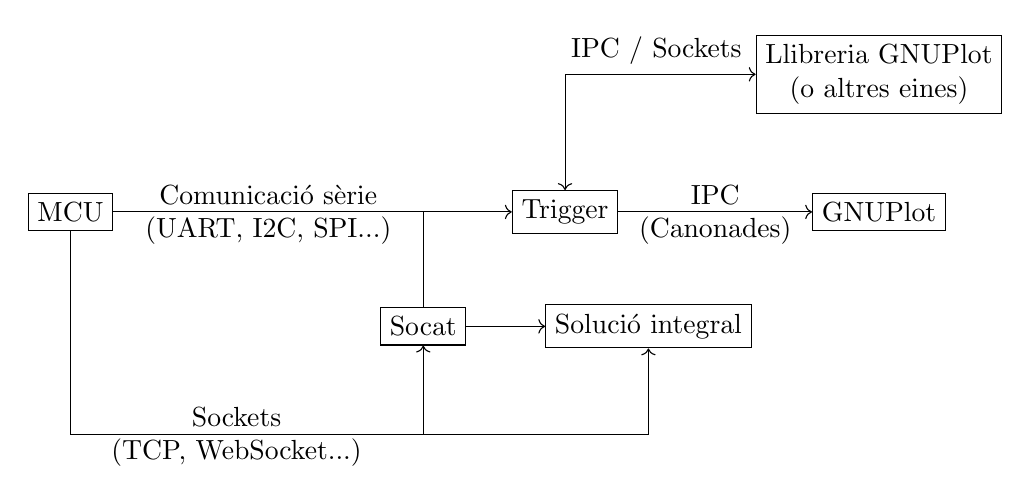
\begin{tikzpicture}
            \node[draw, rectangle] (mcu) {MCU};
            \node[right=of mcu, xshift=8em, minimum height=1.15em] (nexe-serie-socat) {};
            \node[draw, rectangle, align=center, right=of nexe-serie-socat] (trigger) {Trigger};
            \node[draw, rectangle, right=7em of trigger] (gnuplot) {GNUPlot};
            \draw[-] (mcu) -- node[yshift=-0.1em, align=center] {Comunicació sèrie\\(UART, I2C, SPI...)} (nexe-serie-socat.center);
            \draw[->] (nexe-serie-socat.center) -- (trigger);
            \draw[->] (trigger) -- node[yshift=-0.1em, align=center] {IPC\\(Canonades)} (gnuplot);

            \node[draw, rectangle, below=of nexe-serie-socat] (socat) {Socat};
            \node[below=of socat] (nexe-sockets) {};
            \draw[-, to path={|- node[yshift=-0.1em, xshift=6em, align=center] {Sockets\\(TCP, WebSocket...)} (\tikztotarget)}] (mcu) edge (nexe-sockets.center);
            \draw[->] (nexe-sockets.center) -- (socat); \draw (socat) -- (nexe-serie-socat.center);

            \node[draw, rectangle, align=center, above=of gnuplot] (llibreria-gnuplot) {Llibreria GNUPlot\\(o altres eines)};
            \draw[-, to path={|- node[above, xshift=3.3em] {IPC / Sockets} (\tikztotarget)}] (trigger.north) edge[<->] (llibreria-gnuplot);

            \node[draw, rectangle, align=center, right=of socat] (solucio-integral) {Solució integral};
            \node[below=of nexe-serie-socat, yshift=2.1em] (nexe-serie-solucio) {};
            \draw[->] (socat) -- (solucio-integral);
            \draw[-, to path={-| (\tikztotarget)}] (nexe-sockets.center) edge[->] (solucio-integral);
      \end{tikzpicture}
      }
\end{figure}

\section{OsPlot-MCU}

\subsection{Descripció de l'arquitectura}

OsPlot-MCU adopta un enfocament diferent per a la comunicació entre el
microcontrolador i l'ordinador. En aquest cas el programa del
microcontrolador es modifica per implementar el sistema de ``trigger''
directament en el mateix microcontrolador.

\newpage

L'avantatge principal d'aquesta solució és la seva eficiència,
especialment quan el microcontrolador té una capacitat substancial de
processament disponible. D'aquesta manera s'aprofita la totalitat dels
recursos interns del microcontrolador per realitzar el processament
necessari, reduint la càrrega de computació a l'ordinador i alliberant
recursos per altres tasques.

Precisament per això, l'enfocament d'OsPlot-MCU és adequat en
situacions en què es desitja minimitzar la càrrega de computació a
l'ordinador per diversos motius. Per exemple, en aplicacions on s'ha
de considerar l'eficiència energètica o si es vol reduir la
dependència de l'ordinador per a tasques de processament intensives.

\subsection{Extensions}

Com amb OsPlot-PC, OsPlot-MCU ofereix altres opcions per la
comunicació entre el microcontrolador i l'ordinador. A part del port
sèrie, és possible utilitzar altres protocols de comunicació sèrie com
SPI o I2C, o fins i tot comunicació a través de ``sockets''. I també
existeix la possibilitat de fer servir llibreries específiques de
GNUPlot o altres eines per fer gràfiques com les que s'han mencionat a
l'apartat \ref{subsec:extensions-osplot-pc}.

\subsubsection{Comunicació bidireccional amb el microcontrolador}

En l'arquitectura OsPlot-MCU l'algoritme de ``trigger'' s'executa al
microcontrolador, pràcticament forçant a establir una comunicació
bidireccional per permetre l'ajust dels paràmetres del ``trigger''.
Això vol dir que pel port sèrie circularan bytes que no representen
mostres, obligant a establir algun mecanisme per distingir-los.

Una manera senzilla i eficient d'aconseguir-ho és utilitzant un
caràcter d'escapament i enviament per paquets. Per exemple, si prenem
el byte 128 com a caràcter d'escapament, una mostra amb valor 128 es
representaria com 128 i 128, mentre que un final del paquet de mostres
es pot indicar amb els bytes 128 i 0. Altres maneres més elaborades
impliquen l'ús d'eines com
\href{https://protobuf.dev/}{\underline{Protobuf}}, un mecanisme
eficient de serialització que permet estructurar dades per crear un
protocol de comunicació.

\subsection{Diagrama de l'arquitectura}

\begin{figure}[!hb]
      \centering
      \resizebox{\textwidth}{!}{
      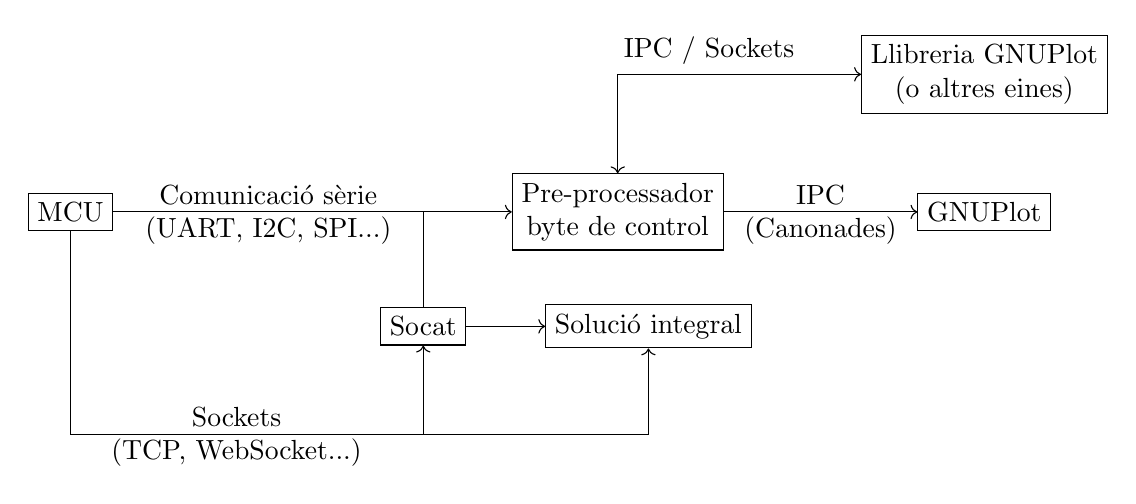
\begin{tikzpicture}
            \node[draw, rectangle] (mcu) {MCU};
            \node[right=of mcu, xshift=8em, minimum height=1.15em] (nexe-serie-socat) {};
            \node[draw, rectangle, align=center, right=of nexe-serie-socat] (trigger) {Pre-processador\\byte de control};
            \node[draw, rectangle, right=7em of trigger] (gnuplot) {GNUPlot};
            \draw[-] (mcu) -- node[yshift=-0.1em, align=center] {Comunicació sèrie\\(UART, I2C, SPI...)} (nexe-serie-socat.center);
            \draw[->] (nexe-serie-socat.center) -- (trigger);
            \draw[->] (trigger) -- node[yshift=-0.1em, align=center] {IPC\\(Canonades)} (gnuplot);

            \node[draw, rectangle, below=of nexe-serie-socat] (socat) {Socat};
            \node[below=of socat] (nexe-sockets) {};
            \draw[-, to path={|- node[yshift=-0.1em, xshift=6em, align=center] {Sockets\\(TCP, WebSocket...)} (\tikztotarget)}] (mcu) edge (nexe-sockets.center);
            \draw[->] (nexe-sockets.center) -- (socat); \draw (socat) -- (nexe-serie-socat.center);

            \node[draw, rectangle, align=center, above=of gnuplot] (llibreria-gnuplot) {Llibreria GNUPlot\\(o altres eines)};
            \draw[-, to path={|- node[above, xshift=3.3em] {IPC / Sockets} (\tikztotarget)}] (trigger.north) edge[<->] (llibreria-gnuplot);

            \node[draw, rectangle, align=center, right=of socat] (solucio-integral) {Solució integral};
            \node[below=of nexe-serie-socat, yshift=2.1em] (nexe-serie-solucio) {};
            \draw[->] (socat) -- (solucio-integral);
            \draw[-, to path={-| (\tikztotarget)}] (nexe-sockets.center) edge[->] (solucio-integral);
      \end{tikzpicture}
      }
\end{figure}

\chapter{Implementació d'OsPlot-PC amb Arduino-C/Python/Chart.js}

En aquesta secció es descriu un exemple d'implementació
d'OsPlot-PC. El programa de l'Arduino és el mateix que s'ha descrit a
l'apartat \ref{programa-arduino-c}. L'algoritme de ``trigger''
s'implementarà utilitzant Python asíncron, i es comunicarà amb una
interfície basada en tecnologia web mitjançant l'ús de WebSockets.

El codi font d'aquesta implementació es pot trobar a
\url{https://github.com/JoanVC100/OsPlot/tree/main/OsPlot-PC}.

\section{``Trigger'' Python amb WebSockets}

\subsection{Descripció de l'algoritme de ``trigger''}
\label{subsec:maquina-trigger}

Per simplicitat, s'ha modelat mitjançant una màquina d'estats un
algoritme de ``trigger normal'' activat per flanc de pujada (sense
disparador automàtic).

La màquina comença en l'estat ``ESPERANT\_TRIGGER'', on compara
successivament les mostres d'entrada amb un nivell de trigger
predefinit. Quan es detecta un flanc de pujada (la mostra actual és
inferior al nivell de trigger i la mostra anterior és igual o superior
al nivell de trigger), la màquina passa a l'estat ``CAPTURANT''.

En l'estat de ``CAPTURANT'' es fa servir un comptador que disminueix a
mesura que arriben les mostres. Un cop es captura un nombre de mostres
determinat (n\_capturades $== 0$), s'envien les mostres a la
interfície i la màquina torna a l'estat d'``ESPERANT\_TRIGGER''.

\begin{figure}[!hb]
      \centering
      \resizebox{\textwidth}{!}{
      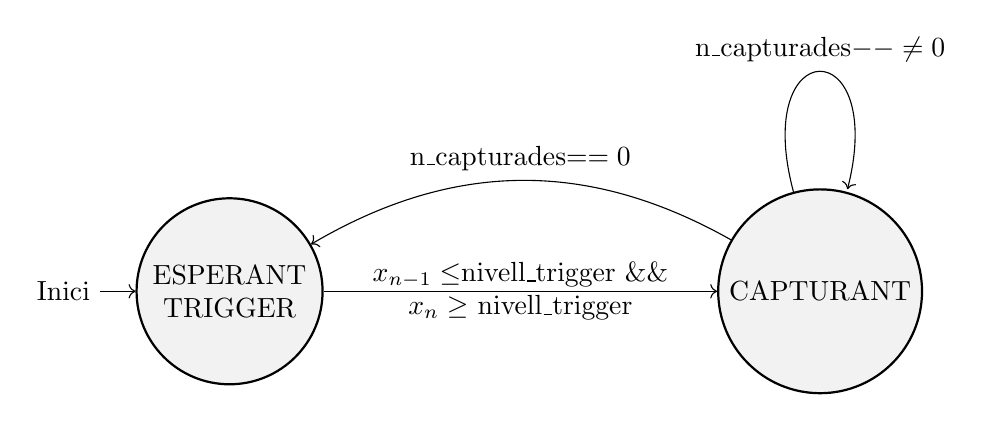
\begin{tikzpicture}[node distance=7.5cm]
            \node[state, initial, align=center] (esperant_trigger) {ESPERANT\\TRIGGER};
            \node[state, right of=esperant_trigger] (capturant) {CAPTURANT};
            \draw (esperant_trigger) edge[->] node[align=center]{$x_{n-1}\leq$nivell\_trigger \&\&\\$x_{n}\geq$ nivell\_trigger} (capturant)
            (capturant) edge[loop above] node[align=center]{n\_capturades$--\neq 0$} (capturant)
            (capturant) edge[bend right, above, ->] node[align=center]{n\_capturades$== 0$} (esperant_trigger);
      \end{tikzpicture}
      }
      \caption{Diagrama de la màquina d'estats del ``trigger''}
\end{figure}

\subsection{Transmissió de les mostres amb WebSockets}

Els \cite[WebSockets]{websockets} són una tecnologia que permet una
comunicació persistent, bidireccional i en temps real entre client i
servidor. Aquesta tecnologia és ideal per rebre les mostres del
``trigger'' i alhora comunicar-se amb el servidor per canviar certs
paràmetres de l'algoritme. En aquest projecte, s'ha utilitzat la
llibreria de Python
\href{https://pypi.org/project/websockets/}{\underline{websockets}},
que està dissenyada per treballar amb Python asíncron
(\href{https://docs.python.org/3/library/asyncio.html}{\underline{asyncio}}).

Primerament, el programa de ``trigger'' ha de cridar a la funció
``websockets.serve()'', que crea un servidor WebSocket per acceptar
peticions de connexions (escoltar al port 26142), i hi associa una
funció que s'executarà per cada connexió entrant.

Aquesta funció afegeix cada connexió en un conjunt global de Python
(un ``set'' global) i entra en un bucle infinit. Dins del bucle
principal, s'encarrega de rebre i gestionar els missatges enviats pels
usuaris, com ara les so\lgem icituds de canvi de paràmetres
específics.

D'altra banda, la màquina d'estats del ``trigger'' fa servir el
conjunt de connexions global per realitzar un ``broadcast'' de les
mostres quan la màquina surt de l'estat ``CAPTURANT'', enviant de
manera efectiva les mostres a tots els clients connectats a través de
WebSockets.

I per simplificar la comunicació entre la interfície i el ``trigger''
s'ha utilitzat ``Protobuf'', que permet canviar els paràmetres de
l'algoritme de ``trigger'' i rebre dades del servidor, com les mostres
capturades. ``Protobuf'' fa servir un format de missatges estructurat
i eficient ($\approx 2$bytes de sobrecàrrega per paquet de mostres),
mantenint una transmissió de dades lleugera pels clients.

\section{Interfície amb Chart.js}

La interfície per visualitzar les mostres de l'osci\lgem oscopi s'ha
desenvolupat utilitzant tecnologia web, fet que permet aprofitar els
avantatges dels ``frameworks'' com ``Tauri'' per crear aplicacions
multiplataforma.

Per la construcció dels gràfics en temps real s'ha utilitzat una
llibreria JavaScript anomenada Chart.js. Aquesta llibreria aprofita
l'element ``canvas'' de HTML5 que permet oferir una experiència visual
atractiva i interactiva, alhora que manté un bon rendiment respecte a
altres alternatives.

A diferència de GNUPlot, es transfereixen directament les mostres a un
``array'' associat al gràfic (en comptes de fer servir cues). Aquest
``array'' conté les dades dels eixos ``x'' i ``y''. Quan arriba un
paquet de mostres a través del WebSocket, es copien totes les mostres
a les ``ys'' i es crida la funció ``update()'' per actualitzar el
gràfic en temps real amb les noves dades.

\chapter{Implementació d'OsPlot-MCU amb Arduino-C/Rust/GNUPlot}

\section{Modificació del programa d'Arduino}

Com a punt de partida, es prendrà el programa desenvolupat a l'apartat
\ref{programa-arduino-c} i s'hi incorporarà la màquina d'estats de
l'apartat \ref{subsec:maquina-trigger} mitjançant un bucle després
d'inicialitzar els perifèrics. A més, s'afegirà la
comunicació bidireccional per permetre canviar els paràmetres del
``trigger'' des de la interfície, mitjançant una altra màquina
d'estats.  I per acabar, s'inclourà un filtre per reduir la freqüència
de mostreig efectiva calculant una mitjana de ``n'' mostres per tal de
reduir el soroll que captura l'ADC.

El codi font d'aquesta implementació es pot trobar a
\url{https://github.com/JoanVC100/OsPlot/tree/main/OsPlot-MCU}.

\subsection{Comunicació bidireccional amb el ``trigger''}

Per a la comunicació bidireccional, s'ha adoptat una estratègia basada
en l'enviament de paquets amb bytes de control per minimitzar el temps
processament de mostres. S'ha implementat una màquina d'estats que, en
l'estat ``MÀQUINA\_TRIGGER'', continua llegint mostres mentre no es
generi una interrupció de recepció de bytes.

Però, quan es produeix la primera interrupció, es para la captura de
mostres i l'Arduino queda en l'estat ``REBRE\_ORDRES'', en espera
d'ordres de l'ordinador. Només es reactiva l'algoritme de ``trigger''
quan s'envia l'ordre ``INICIA\_TRIGGER'' des de l'ordinador.

\begin{figure}[!hb]
      \centering
      \resizebox{\textwidth}{!}{
      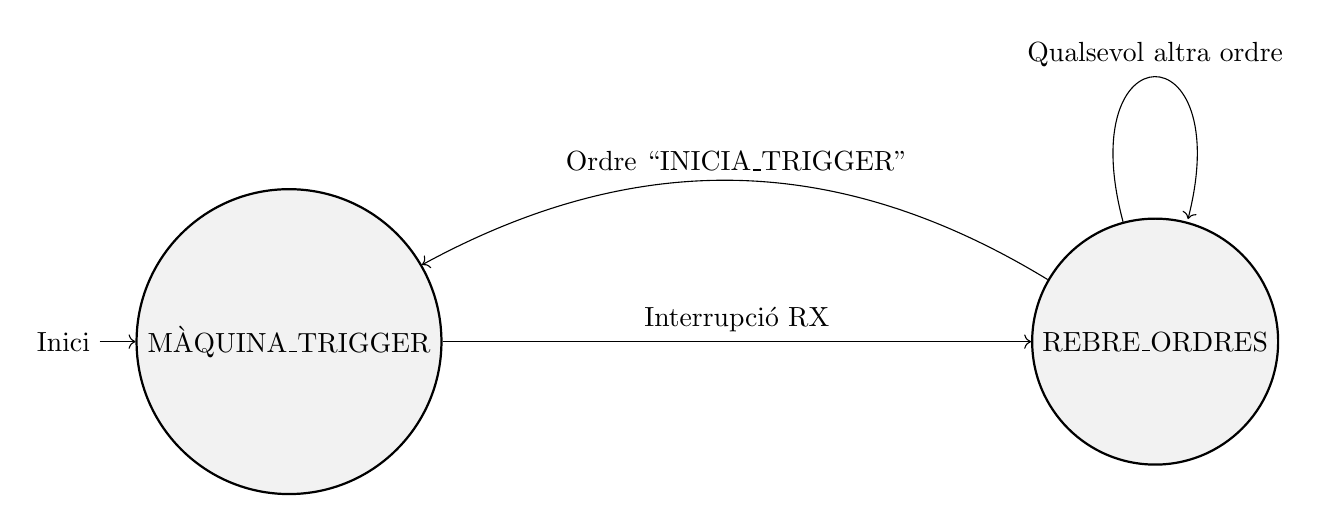
\begin{tikzpicture}[node distance=11cm]
            \node[state, initial] (maquina_trigger) {MÀQUINA\_TRIGGER};
            \node[state, right of=maquina_trigger] (rebre_ordres) {REBRE\_ORDRES};
            \draw (maquina_trigger) edge[->, above] node{Interrupció RX} (rebre_ordres)
            (rebre_ordres) edge[loop above] node{Qualsevol altra ordre} (rebre_ordres)
            (rebre_ordres) edge[bend right, above, ->] node{Ordre ``INICIA\_TRIGGER''} (maquina_trigger);
      \end{tikzpicture}
      }
      \caption{Diagrama de la màquina d'estats per la comunicació bidireccional}
\end{figure}

\clearpage

El protocol de comunicació bidireccional utilitza un byte de control
amb valor 128 seguits d'un byte que indica el tipus de missatge
enviat:

\begin{itemize}
\item MCU\_FINESTRA: Indica el final d'un paquet de mostres. Pot tenir
  qualsevol mida.
\item MCU\_FACTOR\_OVERSAMPLING\_CANVIAT: Indica èxit en canviar el
  nombre de mostres del filtre de mitjana.
\item MCU\_FACTOR\_OVERSAMPLING: És un paquet que conté un byte amb el
  nombre de mostres del filtre de mitjana.
\item MCU\_N\_MOSTRES\_CANVIADES: Indica que el nombre de mostres
  d'una finestra s'ha canviat.
\item MCU\_N\_MOSTRES: Paquet que conté el nombre de mostres d'una
  finestra (2 bytes).
\item MCU\_FS: Retorna la freqüència de mostreig de l'ADC.
\item MCU\_NIVELL\_TRIGGER\_CANVIAT: Indica que el nivell del
  ``trigger'' s'ha canviat.
\item MCU\_NIVELL\_TRIGGER: Retorna un byte amb el nivell de
  ``trigger''.
\item MCU\_ERROR: Aquest missatge indica que s'ha produït un error en
  la comunicació amb l'Arduino. Pot ser causat per una comanda
  incorrecta, valors invà\lgem ids...
\end{itemize}

\subsection{Filtre per reduïr la freqüència de mostreig efectiva}

L'implementació del filtre per reduir la freqüència de mostreig
efectiva utilitza una tècnica de mitjana de ``n'' mostres. Aquesta
tècnica permet mantenir la mateixa freqüència de mostreig, i alhora
reduir el soroll capturat per l'ADC. La freqüència efectiva es calcula
dividint la freqüència de mostreig original pel nombre de mostres
utilitzades en cada càlcul de mitjana ($\frac{F_{s}}{n}$).

Aquest tractament del senyal pot ser útil quan es vol visualitzar
senyals de més baixa freqüència amb més resolucio (> 8 bits), o com a
mètode per augmentar les divisions de temps. Però és important tenir
en compte que aquesta mitjana pot tenir un efecte negatiu en la
captura de pics ràpids. El suavitzament de les fluctuacions pot
provocar que els pics ràpids es redueixin o desapareguin a la
representació gràfica. Aquesta és una limitació inherent de la tècnica
de mitjana, i s'hauria de solucionar amb altres enfocaments, com el
``trigger'' amb detecció de pics.

\section{Programa auxiliar amb Rust}

El programa d'OsPlot-MCU escrit en Rust està orientat a la programació
asíncrona i per esdeveniments. Concretament s'utilitza ``tokio'', una
biblioteca de programació asíncrona per al llenguatge
Rust. Proporciona eines i abstraccions per gestionar aquest paradigma
de programació de manera senzilla. En concret es fa servir l'extensió
``tokio-serial'', que afegeix la possibilitat d'interactuar amb ports
sèrie de manera asíncrona.

\newpage

La tasca principal del programa és una funció que, primer de tot,
inicialitza el port sèrie enviant la comanda per iniciar el
``trigger'' del microcontrolador. Seguit d'això, es crea el procés de
GNUPlot en un directori temporal, que conté la cua per la transmissió
de mostres i el ``script'' que ha d'executar.  Aquest ``script''
inclou alguna modificació, ja que els valors de l'eix ``x'' s'envien
també per la cua, evitant a GNUPlot càlculs per cada representació.

Aquesta tasca entra en un bucle que contínuament llegeix paquets del
port sèrie. Quan arriba un paquet de mostres, les mostres es copien a
un ``array'' que contindrà cada mostra i la seva corresponent ``x'', i
l'enviarà directament a través de la canonada (actualment, per la
resta de paquets no es realitza accions rellevants). Aquest bucle
només podrà acabar quan, o bé hi hagi algún error (es tanca el port
sèrie, mor el procés de GNUPlot...), o si la tasca de la ``CLI'' li
envia un missatge de tancament (per Ctrl-C, ordre de sortida...).

La tasca de la ``CLI'' té com a funció interpetar ordres de l'usuari
(que arriben per ``stdin'') i transmetre-les a la tasca principal.
Per limitacions de ``tokio'', en comptes de crear una tasca per llegir
la ``stdin'', es crea un fil que llegeix l'entrada de l'usuari i
l'envia a la tasca de la ``CLI''. I per gestionar el Ctrl-C, es crea
un altre fil que envia una senyal a la mateixa tasca.

Tota la comunicació entre tasques és possible gràcies als ``MPSC''
(``Multi-Producer Single-Consumer'') i ``Oneshots'', que són canals
asíncrons que permeten la comunicació entre múltiples tasques. Separar
el programa en aquestes tasques permet separar els diferents blocs
d'esdeveniments d'una manera clara i estructurada.

\chapter{Línies futures}

\section{Múltiples esdeveniments de ``triggers'' per ``frame''}

En buscar la simplicitat, les implementacions realitzades en el
treball no tenen en compte la visualització de múltiples esdeveniments
de ``trigger'' en un únic ``frame''.  Tota informació que no pugui ser
representada en el transcurs de dos ``frames'' consecutius es
descarta.  Això significa que, en casos on la freqüència del senyal és
alta i hi ha una gran quantitat d'esdeveniments de ``trigger'' per
temps de ``frame'', l'observador pot perdre moltes dades rellevants i
no ser capaç de discernir tots els esdeveniments que s'han produït en
el transcurs d'un ``frame''.

Els osci\lgem oscopis professionals tenen en compte aquesta limitació
i implementen solucions per superar-la. Un enfocament comú és
utilitzar una representació visual que permet mostrar tots els
disparaments generats en el transcurs d'un ``frame''
determinat. Aquesta tècnica implica assignar una transparència
variable als esdeveniments de ``trigger'', de manera que les ones més
antigues apareguin més transparents, mentre que les ones més recents
es mostren més clares i destacades. Aquesta representació visual
proporciona una indicació de la forma i la tendència del senyal al
llarg del temps sense augmentar la capacitat de visualització de la
pantalla.

Amb aquesta tècnica, l'observador pot identificar si hi ha hagut
picades o canvis significatius en el senyal durant el ``frame'', així
com observar si el senyal és estable o no. Aquesta informació és
valuosa per a l'anàlisi i la comprensió del comportament del senyal en
situacions en què hi ha múltiples esdeveniments de ``trigger'' en un
període de temps que la pantalla de l'osci\lgem oscopi no podria
representar (o fins i tot, que l'ull humà no podria apreciar).

\section{Plantejar alternatives al port sèrie}

En el marc d'aquest treball, s'ha observat que es pot arribar
ràpidament al límit de velocitat del port sèrie. Amb una taxa d'ADC
estable d'aproximadament 76.000 mostres per segon, utilitzar una
velocitat de transmissió d'1 Mbps (100.000 mostres per segon) comença
a ser insuficient per acomodar el flux de dades de l'osci\lgem
oscopi. Si es pogués augmentar la velocitat de mostreig de l'ADC a
l'Arduino, el port sèrie deixaria de ser una opció viable, ja que una
velocitat de 2 Mbps resultaria molt més inestable que 1 Mbps,
velocitat la qual ja és fora de l'estàndard.

En vista d'aquesta limitació, cal explorar alternatives. Per exemple,
es podria fer servir SPI, que permet una velocitat màxima de fins a 60
Mbps en alguns casos, sense experimentar una càrrega excessiva. Això
implicaria un augment significatiu en la taxa de mostreig teòrica,
arribant a un màxim de 7,5 milions de mostres per segon.

Una altra opció a considerar seria buscar mètodes de comunicació
directa a través de la interfície USB, evitant conversions de port
sèrie a USB i a l'inrevés (com és el cas de l'Arduino). El programa a
l'ordinador podria accedir directament a l'USB, augmentant molt més
les velocitats de transmissió teòriques, segons l'estàndard USB
utilitzat.

\section{Inclusió de SDR a l'arquitectura}

Una altra línia futura interessant a explorar és l'ús de \cite[Ràdio
  Definida per Software]{viqui-sdr} en l'arquitectura OsPlot. En lloc
d'utilitzar protocols serials tradicionals com UART o SPI, així com
altres tecnologies de xarxa com TCP/IP o WebSockets, l'ús de SDR pot
proporcionar una solució més versàtil per a la lectura, el
processament i l'enviament de mostres.

Les SDR són dispositius que permeten capturar, processar i transmetre
senyals de ràdio mitjançant programari. A diferència dels sistemes de
ràdio tradicionals, que utilitzen components electrònics
especialitzats per a funcions específiques, les SDR es basen en
plataformes programables i flexibles que utilitzen processament
digital de senyals per dur a terme diverses tasques de comunicació.
Mitjançant l'ús de programari és possible canviar i adaptar els
paràmetres i funcions de les SDR, com la modulació, la freqüència i la
codificació, per adaptar-se a diferents aplicacions i requisits.

S'hauria d'investigar com integrar-los a l'arquitectura OsPlot per
intentar aprofitar les seves capacitats de processament digital. Una
SDR permet capturar senyals analògics, convertir-los en senyals
digitals i processar-los mitjançant algoritmes de processament de
senyal digital. Això obriria la porta a una gran varietat de tècniques
de modulació, codificació i descodificació que podrien ser utilitzades
per a la transmissió de mostres. També s'hauria d'investigar l'ús de
diferents bandes de freqüència que es podrien fer servir per a una
millor transmissió de les mostres.

\chapter{Conclusions}

\printbibliography

\end{document}

%%% Local Variables:
%%% mode: latex
%%% TeX-master: t
%%% LaTeX-biblatex-use-Biber: t
%%% End:
